\clearpage
\section*{Execute}
The Execute stage takes \verb+iCode+, \verb+iFun+, \verb+valA+, \verb+valB+, and \verb+valC+ along with the clock signal as inputs and outputs \verb+valE+. 
 Additionally, the Sign Flag, Overflow Flag, and the Zero Flag are set during this stage.\\\\
 \verb+iCode+, \verb+valA+, \verb+valB+, and \verb+valC+ are fed into \verb+CTRLogic+, which uses the information regarding the current instruction to send into the ALU the two values on which an operation is to be executed. \\\\
 \verb+ifun+ and \verb+icode+ are fed into ALUFun to generate a 2 bit output, \verb+noCodenoFun+, to communicate to the ALU which operation to execute.\\\\
 The ALU takes in 3 inputs, \verb+A+, \verb+B+, and \verb+notFun+, and computes the necessary operation (between addition, subtraction, logical AND, and logical XOR).  The output is sent out to \verb+ValE+ and stored in a register, and the flags are set in \verb+pcc+.\\\\
 setCC takes in \verb+iCode+ in order to determine if the flag should be set on this operation or not.  This output, along with both the clock and the flag outputs, are fed into CC in order to set the flag.  This output is then used to set the jump condition in combination with \verb+ifun+, to be used later in PCUpdate.
\subsection*{Contributors}
Arjun Kurkal
\clearpage
\subsection*{Screenshots}

\begin{figure}[!ht]
    \centering
    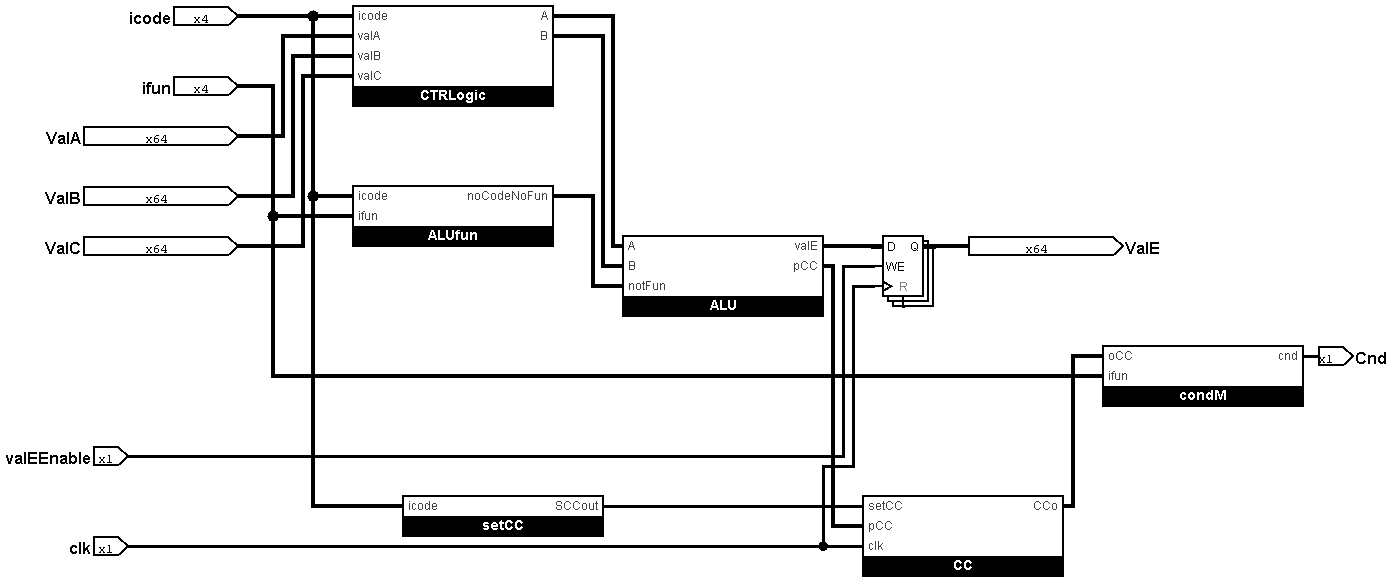
\includegraphics[width=\textwidth]{Images/Execute.png}
    \caption{Execute}
\end{figure}
